\subsection{图像生成模型结构总览}

该部分作为废案的暂存地。

目前存在一些能够生成令人印象深刻的图像的模型,如Stable Diffusion\cite{rombachHighResolutionImageSynthesis2022a}、DALL-E\cite{rameshHierarchicalTextConditionalImage2022}、Imagen\cite{saharia2022photorealistic}等。

Stable Diffusion\cite{rombachHighResolutionImageSynthesis2022a}能够生成高质量的图像。它广泛应用于图像生成、图像修复、图像超分辨率、艺术创作和游戏设计等领域,具有高灵活性和优秀的图像生成能力。Stable Diffusion 在机器学习和计算机视觉领域内被广泛使用,是一款强大的图像生成工具,其网络模型如图\ref{img_stable}所示。

\begin{figure}[htbp]
    \centering
    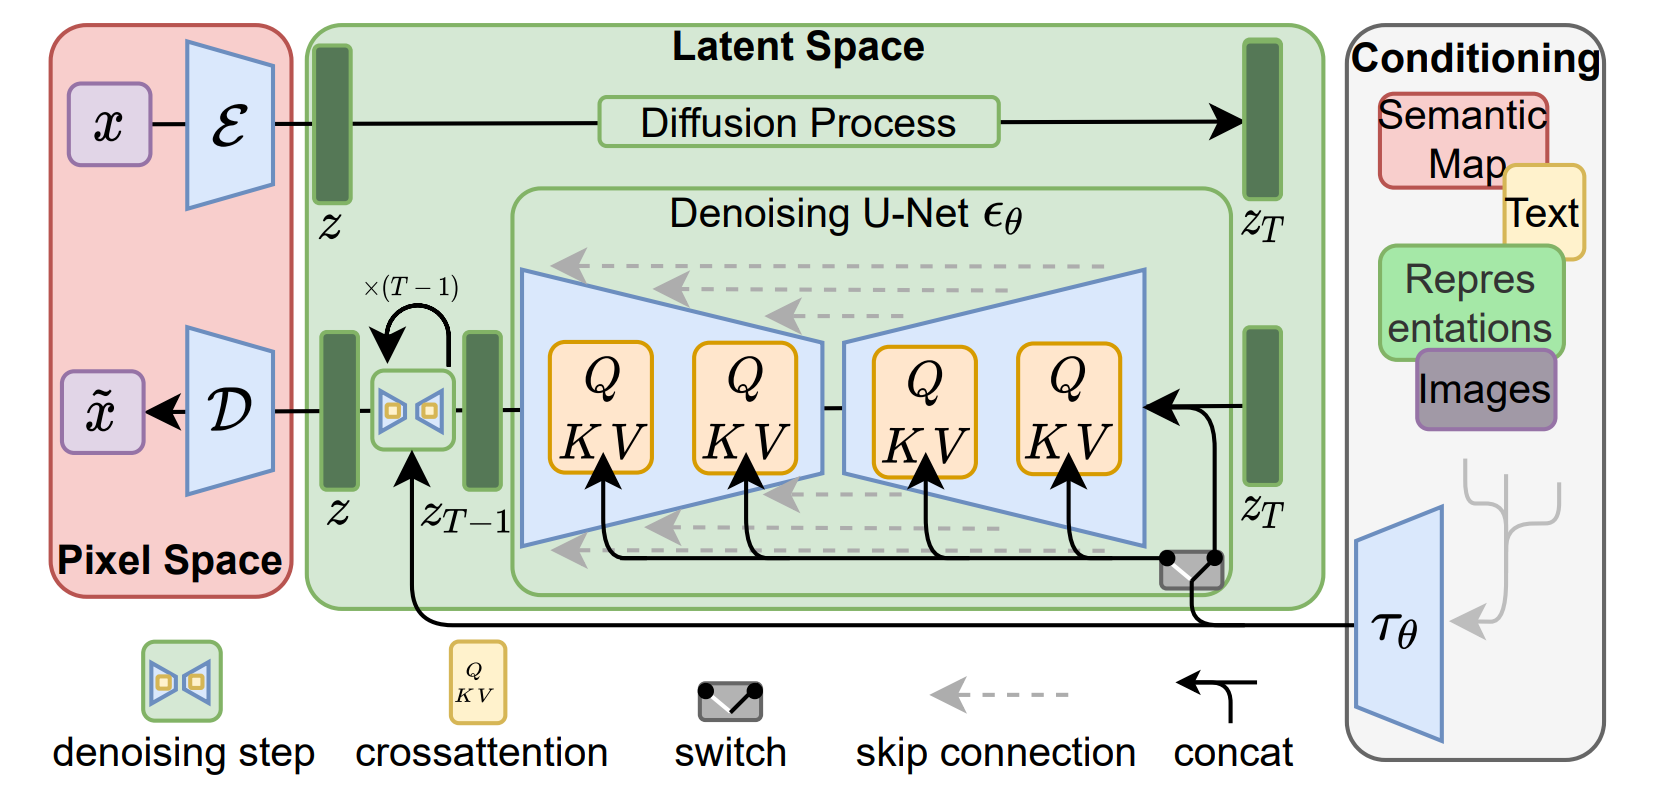
\includegraphics[width=0.8\textwidth]{SD.png}
    \caption{Stable Diffusion的网络结构\cite{rombachHighResolutionImageSynthesis2022a}}
    \label{img_stable}
\end{figure}

DALL-E\cite{rameshHierarchicalTextConditionalImage2022} 是一个由OpenAI开发的基于深度学习的图像生成模型。其核心技术是生成式对抗网络(GAN)和变分自编码器(VAE),能够从文本描述生成高质量的图像。DALL-E 能够理解并结合复杂的自然语言描述,生成与描述内容相对应的图像。它广泛应用于图像生成、创意设计、广告制作和内容创作等领域,展示了强大的生成能力和多样性。DALL-E 的出现为人机交互和自动化创意设计提供了新的可能性,受到广泛关注和应用。其网络模型如图\ref{img_dalle}所示。

\begin{figure}[htbp]
    \centering
    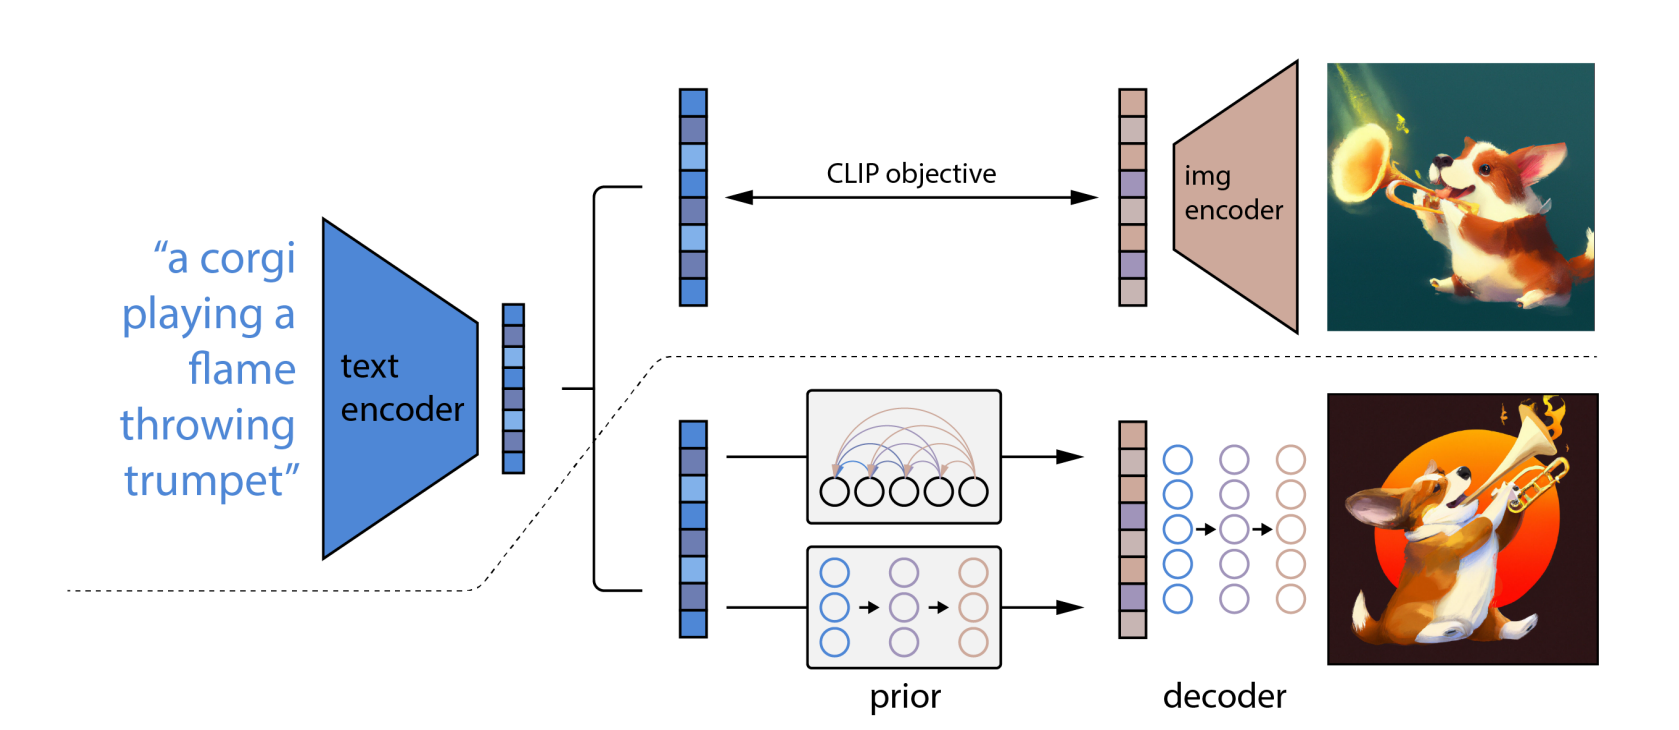
\includegraphics[width=0.8\textwidth]{DALLE.png}
    \caption{DALLE的网络结构\cite{rameshHierarchicalTextConditionalImage2022}}
    \label{img_dalle}
\end{figure}

观察以上两个当前最为流行的图像生成模型,可以发现他们采样了类似的结构:文字编码模块-图像生成模块-图像解码模块,这三个模块协同工作,可以认为是当前最先进的图像生成模型的基本结构,可以绘制成如下基本结构图。

『缺少基本图像』

